\documentclass{article}
\usepackage[utf8]{inputenc}
\usepackage[english]{babel}
\usepackage[a4paper,top=2cm,bottom=2cm,left=3cm,right=3cm,marginparwidth=1.75cm]{geometry}
\usepackage{amsmath}
\usepackage{graphicx}
\usepackage{hyperref}
\usepackage{csquotes}
\usepackage[style=apa]{biblatex}
\addbibresource{sample.bib}



\title{SIF3004 Final Year Project Proposal : RAdio Galaxy Environment Reference Survey (RAGERS) Project }
\author{Lim Ming Kang U2004991/1\\[0.3cm]{Supervisor: Prof. Dr. Zamri Zainal Abidin}}

\begin{document}
\maketitle
\section{Problem Statement}

At the cosmological redshift of $2 < z < 3$ (observing the condition about 10.9 bllion years ago), the universe is actively producing new stars, with highest average star forming rates (SFRs). This period known as "the cosmic noon"\parencite{Schreiber2020}. Galaxies known as "Dusty Star Forming Galaxies (DSFGs) are enriched with dust that serves as the materials to forming stars.
\medskip

\noindent A comprehensive understanding of those galaxies is important in understanding galaxy formation and evolution in the early universe.\parencite{Geach2016}
\medskip

\noindent Characterisation of the region where the aforementioned galaxies reside (galaxy overdensities) with redshift, and the effect of Active Galatic Nuclei (AGN) activity on the growth of the central overdensities are to this day still not thorough.\parencite{ragers2021}
\medskip

\noindent Obscured by dust, those galaxies are not feasible to be observed in visible region, a telescope capable in observing in far infrared wavelength is needed to detect the galaxies.
\medskip

\noindent Raw telescope data needs to be reduced, cleaned and calibrated before doing analuysis, as noise and false detections may be presence, the processes are essential to obtain a clean map for analysis. 

\medskip

\noindent The addition of far infrared data would is significant to multiwavelength analysis of galaxies especially in obtaining photometric redshift.

\section{Objectives}
\begin{enumerate}
    \item To study statistically (eg. surface number density) of galaxy overdensities in a source field.
    \item To analyse and compare protocluster at high redshift with galaxy cluster in local universe.
    \item To obtain photometric redshift of submm galaxies in a source field using multiwavelength analysis.
\end{enumerate}
\section{Background}
Galaxies in the universe can be classified based on their morphologies (or shapes). The famous hubble tuning fork is a classification scheme that mainly divides galaxy morphologies into two categories which are ellipticals and spirals. It is oversimplified with the discovery, although not abundant, of irregular galaxies \parencite{Gallagher1984}. However, at high redshift, the limitation of optical observation and image resolution places a challenge on measured morphologies \parencite{Rouan2008}. Galaxies are then categorised based on wavelength of energetic emission. For instances radio galaxies emit relatively high radio frequency than its optical counterpart. Likewise, submillimetre galaxies emit strong electromagnetic wave at submillimetre region.
\medskip

\noindent As one of the massive structures of the universe, The evolution of galaxies gives insights to the evolution
of the universe. Population of galaxies based on types in certain redshift and their star formation rate (SFR) are two parameters to examine the evolution \cite{Martin2005}. Observation has shown that SFR across the history of universe peaks at $2 < z < 3$, this period is known as the cosmic noon. (refer to figure \ref{fig:cosmicnoon}) Light from distance object (eg. a galaxy) undergoes redshifting due to expansion of the universe, therefore allows astrophysicists to observe the "snapshot" of the object at particular history of time, up until young universe (several million years after the big bang \cite{Jiang2021}).  By observing galaxies at high redshift, high population of giant galaxies are particularly interesting to study, such as submillimetre galaxies and high redshift radio galaxies \cite{Singh2014} \cite{Chapman2005},  that contribute to high SFR during "cosmic noon".
\medskip

\noindent Submillimetre Galaxies (SMGs) are rare galaxies with high star formation rates $(>100M_\odot yr^{-1})$ \parencite{DaCunha2021} populated in high redshift region. Suspected to be the progenitors of local massive galaxies \parencite{Casey2014}, SMGs are valuable candidates to study evolution of galaxies in high redshift. One challenge in observing SMGs is the amount of dust, which serves as the building blocks for star formation, which obscure visible light, thus are hard to be observed with optical telescopes. However, the dust absorbs the radiation emitted from new stars and reemmits as far infrared wavelength \parencite{Casey2014}, the observation of SMGs is possible with submillimetre telecopes. 
\medskip

\noindent To solve the aforementioned issue, there have been telescopes operating at far infrared. For instances the Atacama Large Millimeter Array (ALMA) telesope located in northern Chile, Fred Young Submillimeter Telescope, Caltech Submillimeter Observatory (CSO), William Herschel Telescope (WHT)\parencite{Phillips2013} and SCUBA-2 at James Clerk Maxwell Telescope (JCMT), whose data is used in the research of this proposal. They are built at high attitude, usually on top of the mountains (eg. JCMT at Mauna Kea, Hawaii(~4092m)) to minimize the attenuation of incoming signal by the Earth atmosphere.\parencite{Phillips2013}
\medskip

\noindent At high redshift, observation has shown overdensities of SMGs happen within the vicinity of a High Redshift Radio Galaxy (HzRG), a galaxy emmiting powerful radiowaves. Suspected to be a protocluster (a galaxy cluster at its young age), the dynamic between SMGs and HzRGs can be studied so have a more robust understanding of evolution of masive structure of the universe.\parencite{Saxena2018}

\section{Research Methodology}

The research will be carried out on handling raw 0.85mm and 0.45mm data collected from JCMT SCUBA-2 under RAGERS Project, in collaboration with RAGERS Malaysia Team (from where the raw data is acquired). Data Reduction is run on Starlink software. The process of data handling is shown in Figure \ref{fig:flowchart1}
\medskip

\noindent James Clerk Maxwell Telescope (JCMT) is a 15m telesope designed to run on submillimetre wavelength (far infrared region). It is positioned at Maunakea, Hawaii. 
\medskip

\noindent SCUBA-2 is a camera attached on JCMT to observe at 450$\mu m$ and 850$\mu m$ (~666GHz and 353GHz), which are frequencies emitted by light molecules containing hydrogen (eg. $H_2O,CH$) from the dust \parencite{Phillips2013}. The data is formatted and stored in .sdf format, which is readable by starlink software.
\medskip

\noindent The RAdio Galaxy Environment Reference Survey is a JCMT program to observe overdensities within the Mpc region of 33 radio galaxies at redshift range $1 < z < 3.5$ and mass range $M\ast >=1010.8M\odot $ \parencite{ragers2021}
\medskip

% \noindent Source field is a region spanning across few Mpc centered around a HzRG, which is located at $1 < z < 3.5$ 
% \medskip

\noindent 5C7269 is a source field centered around a HzRG named 5C7269, which is located at $RA = 8h28m39s$, $DEC = 25d28m27.1s$ and $z = 2.218$, 
\medskip

\noindent Starlink is a software consisting of several packages used to reduce and analyse data recorded by SCUBA-2 telescope, including (but not limited to) SMURF for data reduction and GAIA for data visualisation. Telescopes are usually associate with their proprietery software for data handling. For instances, CASA for ALMA, Starlink for JCMT and AIPS for Very Large Baseline Array (VLBA). It is extremely important to produce useful science data from noisy telescope data to remove as much noises as possible (eg. Radio Frequency Inteference (RFI)) and extract useful information to the max. Figure \ref{fig:reducevsunreduce} shows an example of the comparison between raw telescope data, and image after data reduction.

\begin{figure}
    \centering
    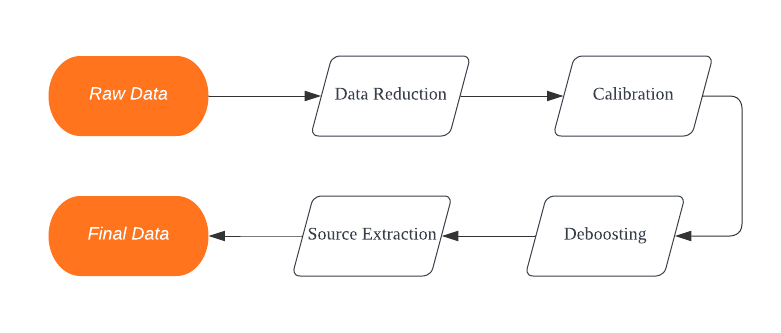
\includegraphics[width=100mm]{Flowchart.png}
    \caption{General process of data handling of raw telescope data.}
    \label{fig:flowchart1}
\end{figure}

\begin{figure}
    \centering
    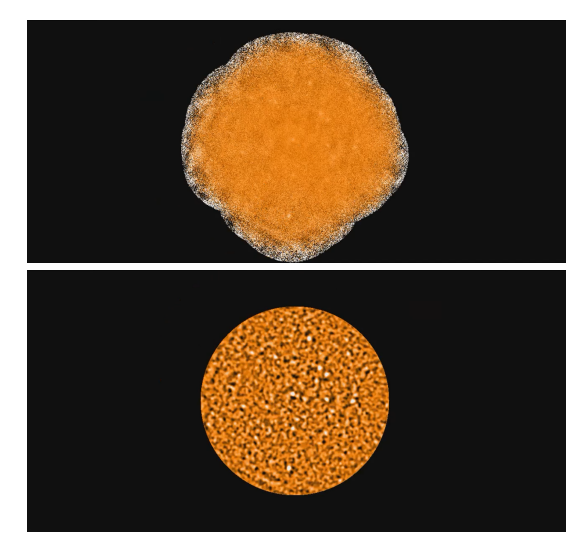
\includegraphics[width=100mm]{reducevsunreduce.png}
    \caption{An example of the comparison between raw telescope data (up), where there is no clear galaxies count, and image after data reduction (down), where SMGs appear as white dots. Source: Thomas R. Greve, private communication.}
    \label{fig:reducevsunreduce}
\end{figure}

\begin{figure}
    \centering
    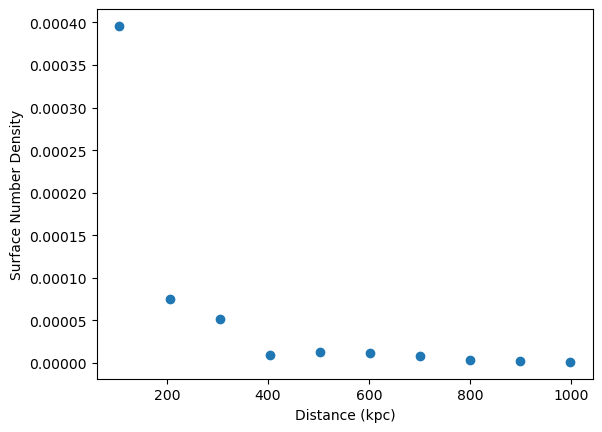
\includegraphics[width=100mm]{SNDensity.png}
    \caption{Surface number density as the function of distance from cluster center}
    \label{fig:sndensity}
\end{figure}

\begin{figure}
    \centering
    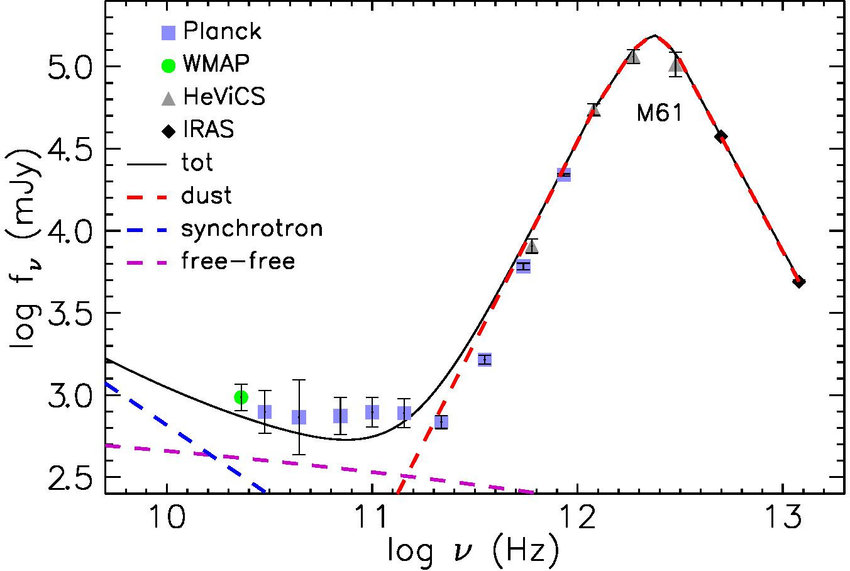
\includegraphics[width=100mm]{SED.png}
    \caption{An example of Spectral Energy Density graph, a logarithmic graph of flux density vs frequency. Source \parencite{Zotti2018}}
    \label{fig:sedgraph}
\end{figure}

\begin{figure}
    \centering
    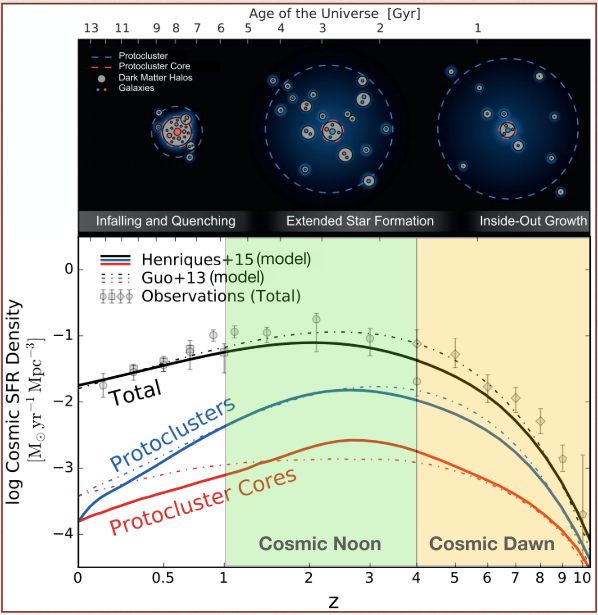
\includegraphics[width=100mm]{cosmic noon.png}
    \caption{Graph of logarithm of cosmic SFR density vs redshift, peaks at around $z = 2$. Source Source: Thomas R. Greve, private communication. and \parencite{Zotti2018}}
    \label{fig:cosmicnoon}
\end{figure}


\section{Expected Results}
A reduced, low noise data similar to figure \ref{fig:reducevsunreduce}b should be obtained. From the reduced data, surface number density as the function of radius from center HzRG can be calculated from the number counts. Figure \ref{fig:sndensity} shows one example of graph of surface number density of cluster galaxies vs distance from a cluster center. A Spectral Energy Density (SED) of each detected submm galaxy can be calculated by combining multiwavelength flux density to obtain photometric redshift. An example of the stated graph is shown in figure \ref{fig:sedgraph}, obtained from article \parencite{Zotti2018}

\section{Significance}
Surface number density is essential in studying the effect of HzRG on the environment. The addition of 0.85mm and 0.45mm in SED will give a more accurate photometric redshift of galaxies, which is crucial to study the evolution of galaxies with redshift. More comprehensive data of proto-cluster dynamic will probe into a more robust understanding of galaxies structure evolution.

\section{Gantt Chart}
\begin{figure}[h]
    \centering
    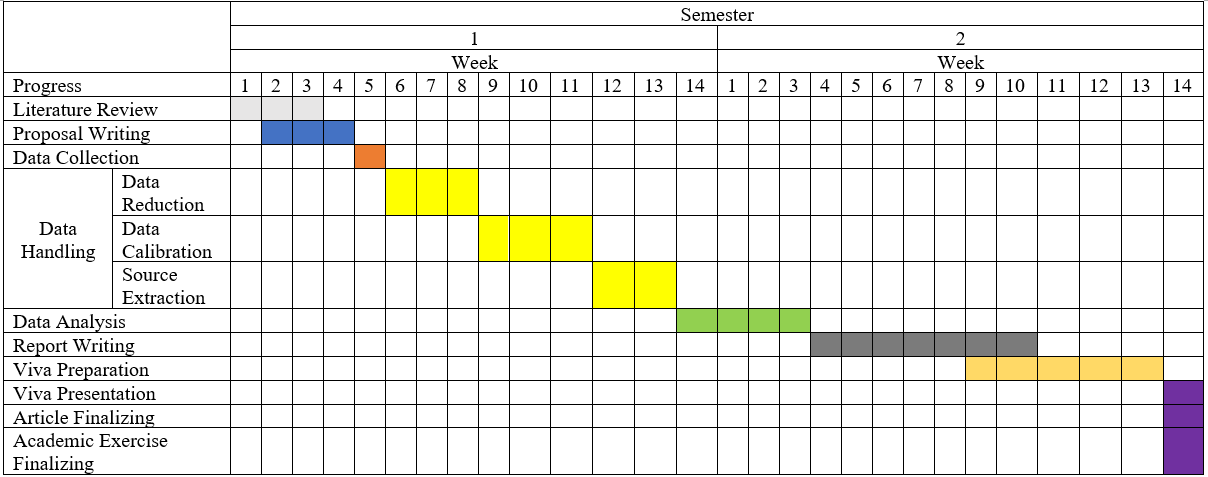
\includegraphics[width=150mm]{gantt chart.png}
    \caption{Gantt Chart of final year project spanning across two semesters, with 1 month of break in between.}
    \label{fig:ganttchart}
\end{figure}

\printbibliography

\end{document}